% ****** Start of file apssamp.tex ******
%
%   This file is part of the APS files in the REVTeX 4.1 distribution.
%   Version 4.1r of REVTeX, August 2010
%
%   Copyright (c) 2009, 2010 The American Physical Society.
%
%   See the REVTeX 4 README file for restrictions and more information.
%
% TeX'ing this file requires that you have AMS-LaTeX 2.0 installed
% as well as the rest of the prerequisites for REVTeX 4.1
%
% See the REVTeX 4 README file
% It also requires running BibTeX. The commands are as follows:
%
%  1)  latex apssamp.tex
%  2)  bibtex apssamp
%  3)  latex apssamp.tex
%  4)  latex apssamp.tex
%
\RequirePackage{lineno}
\setlength{\linenumbersep}{6pt}

\documentclass[%
reprint,
%superscriptaddress,
%groupedaddress,
%unsortedaddress,
%runinaddress,
%frontmatterverbose, 
%preprint,
showpacs,preprintnumbers,
%nofootinbib,
%nobibnotes,
%bibnotes,
 amsmath,amssymb,
 aps,
%pra,
%prb,
%rmp,
%prstab,
%prstper,
%floatfix,
]{revtex4-1}

\usepackage{graphicx}% Include figure files
\usepackage{dcolumn}% Align table columns on decimal point
\usepackage{bm}% bold math
\usepackage{xspace}	% Include xspace
\usepackage{color}
\usepackage{xcolor}
%\usepackage{hyperref}% add hypertext capabilities
%\usepackage[mathlines]{lineno}% Enable numbering of text and display math
%\linenumbers\relax % Commence numbering lines

%\usepackage[showframe,%Uncomment any one of the following lines to test 
%%scale=0.7, marginratio={1:1, 2:3}, ignoreall,% default settings
%%text={7in,10in},centering,
%%margin=1.5in,
%%total={6.5in,8.75in}, top=1.2in, left=0.9in, includefoot,
%%height=10in,a5paper,hmargin={3cm,0.8in},
%]{geometry}

\newcommand{\pt}{\mbox{$p_T$}\xspace}
\newcommand{\raa}{\mbox{$R_{\rm AA}$}\xspace}
\newcommand{\raap}{\mbox{$R_{\rm AA}^{N_{\rm part}}$}\xspace}
\newcommand{\Npart}{\mbox{$N_{\rm part}$}\xspace}
\newcommand{\Ncoll}{\mbox{$N_{\rm coll}$}\xspace}
\newcommand{\Nch}{\mbox{$N_{\rm ch}$}\xspace}
\newcommand{\Et}{\mbox{${\rm E}_T$}\xspace}
\newcommand{\meanpt}{\mbox{$\langle p_T \rangle$}\xspace}
\newcommand{\meanet}{\mbox{$\langle {\rm E}_T \rangle$}\xspace}
\newcommand{\mNcoll}{\mbox{$\langle N_{\rm coll} \rangle$}\xspace}
\newcommand{\sqs}{\mbox{$\sqrt{s}$}\xspace}
\newcommand{\sqsn}{\mbox{$\sqrt{s_{_{NN}}}$}\xspace}
\newcommand{\dau}{\mbox{$d$+Au}\xspace}
\newcommand{\dpb}{\mbox{$d$+Pb}\xspace}
\newcommand{\pau}{\mbox{$p$+Au}\xspace}
\newcommand{\pal}{\mbox{$p$+Al}\xspace}
\newcommand{\hau}{\mbox{$^3\text{He}$+Au}\xspace}
\newcommand{\pp}{\mbox{$p$+$p$}\xspace}
\newcommand{\ppb}{\mbox{$p$+Pb}\xspace}
\newcommand{\pa}{\mbox{$p+A$}\xspace}
\newcommand{\rdau}{\mbox{$R_{dAu}$}\xspace}
\newcommand{\pda}{\mbox{$p(d)+A$}\xspace}
\newcommand{\rpda}{\mbox{$R_{p(d)+A}$}\xspace}
\newcommand{\bbceta}{\mbox{$3.0<|\eta|<3.9$}\xspace}

\bibliographystyle{unsrt}

\linenumbers

\begin{document}

\title{Measurement of Long-Range Angular Correlations and Azimuthal Anisotropies in High Multiplicity \pau Collisions at \sqsn = 200 GeV}% Force line breaks with \\

\author{Author list: Brant will insert later}

\date{\today}% It is always \today, today,
             %  but any date may be explicitly specified

\begin{abstract}
We present the first measurements of long-range azimuthal correlations and the transverse momentum dependence of elliptic flow $v_2$ in high- multiplicity central \pau collisions at \sqsn = 200 GeV. A comparison of these results with those previously measured in central \dau and \hau demonstrates the direct relation between $v_2$ and the initial eccentricity $\varepsilon_2$. Such observation allows us to ascertain the role of the initial geometry as a major driver of collective behavior in small systems, precluding theoretical explanations based on momentum-space domain correlations. Good agreement is observed between the measured $v_2$ and hydrodynamic calculations for all systems. The set of measurements leverages the differential intrinsic geometry of the systems under considerations, to provide stringent constraints for the theoretical determination of medium properties.

\end{abstract}

\pacs{25.75.Dw}% PACS, the Physics and Astronomy
                             % Classification Scheme.
%\keywords{Suggested keywords}%Use showkeys class option if keyword
                              %display desired
\maketitle
% * <shengli.huang@vanderbilt.edu> 2016-07-07T15:24:45.421Z:
%
% ^.
% * <shengli.huang@vanderbilt.edu> 2016-07-07T15:23:55.161Z:
%
% ^.
The azimuthal momentum anisotropy relative to the reaction plane, as quantified by the Fourier coefficients $v_n$ of the azimuthal yield of final state particles, has long been considered evidence for the formation of a strongly interacting, fluid-like quark-gluon plasma (QGP) in A+A collisions~\cite{Snellings:2011sz}. Viscous hydrodynamics supports a picture in which initial spatial inhomogeneities and fluctuations in energy density are translated into final-state momentum anisotropies.  The success of this model~\cite{Luzum:2008cw} in describing bulk observables of the QGP has grounded the concept of hydrodynamic flow as the main driver of the vn signal.

However, recent analyses of \dau and \hau at \sqsn = 200 GeV~\cite{adare_measurement_2014,Adamczyk:2014fcx,PhysRevLett.115.142301} at the Relativistic Heavy-Ion Collider (RHIC), and \ppb at \sqsn = 5.02 TeV and $p+p$ at \sqsn = 7 and 13 TeV~\cite{alice_long_2013,atlas_observation_2012,cms_observation_2012,Khachatryan:2015lva,Aad:2015gqa} at the Large Hadron Collider (LHC) have demonstrated the existence of the same azimuthal anisotropy signals commonly interpreted as evidence of collective behavior in larger systems. Notably, a feature known as \textit{the ridge} has been observed, consisting of a near-side (i.e., around $\Delta \phi = 0$) enhancement in the azimuthal two-particle correlation even when accounting for non-flow contributions. This results in substantial elliptic ($v_2$), and triangular ($v_3$) flow coefficients being measured in these systems.

Although these observations support the idea of QGP formation in small systems, it is not clear whether viscous hydrodynamics applies to this situation since any QGP formed in small systems is not expected to exist long enough for final-state anisotropies to develop as a consequence of hydrodynamic flow. Thus, other explanations have been proposed, including initial state effects from glasma diagrams~\cite{dusling_azimuthal_2012} and partonic scattering in \textsc{ampt}~\cite{bzdak_elliptic_2014,ma_long-range_2014,Koop:2015wea}. A key experimental test to resolve the issue consists in varying the intrinsic initial geometry of the system, and hence of the formed QGP, to analyze the extent to which it is translated to the final state~\cite{nagle_exploiting_2013}. 

The PHENIX collaboration has actively pursued this idea by analyzing data from intrinsically elliptic (\dau)~\cite{adare_measurement_2014,PhysRevLett.111.212301} and triangular (\hau)~\cite{Adare:2015ctn} collision systems at \sqsn = 200 GeV. Viscous hydrodynamics has been found to accurately reproduce the measured $v_n$~\cite{Romatschke:2015gxa} for these systems, establishing the relevance of the initial geometry and hydrodynamic flow in the development of the $v_n$ signal in smaller systems.

This communication completes the above suite of studies by presenting two-particle correlations and the transverse momentum (\pt) dependence of $v_2$ for central \pau collisions at \sqsn = 200 GeV. These results are compared to those from \dau and \hau at a comparable multiplicity, and to available theoretical calculations.

A detailed description of the PHENIX detector system can be found in Ref.~\cite{Adcox2003469}. For this analysis, charged particles were reconstructed with the two central arm spectrometers, each covering $|\eta|<0.35$ and $\pi/2$ in azimuthal angle, consisting of drift chambers and multi-wire proportional pad chambers (PC). Drift chamber tracks are matched to hits in the third layer of the PC, thus limiting the contribution of tracks from decays and photon conversions. The beam-beam counters (BBC) comprise two arrays of 64 quartz radiator \v{C}erenkov detectors, located longitudinally $\pm$1.44 m away from the center of the interaction region (IR), covering $2\pi$ in azimuth and \bbceta. The FVTX detector comprises two identical end-cap assemblies symmetrically located in the longitudinal direction around the IR, covering $1.0 < |\eta| < 3.0$. Charged particles are detected with an efficiency of over 95\% using clusters of hits. The event planes are measured in the Au-going direction using the south BBC (BBC-S) covering $−3.9 < \eta < −3.0$, as well as the reconstructed clusters in the south end-cap of FVTX (FVTX-S) covering $−3.0 < \eta < −1.0$. A $\pm$30 cm event vertex cut was applied for all analyses, corresponding to the central arm acceptance. 

The \pau data set for this analysis was collected during the 2015 run of the PHENIX experiment. It consists of 0.84 billion minimum bias (MB) triggered events and 1.4 billion high-multiplicity (HM) triggered events. The MB trigger is defined as a coincidence between the Au-going and proton-going BBC detectors, requiring at least one photomultiplier tube (PMT) firing in each; in this way 84$\pm$4\% of the total inelastic \pau cross section is captured. The HM trigger is based on the MB trigger, but imposes the additional requirement of more than 48 photomultiplier tubes firing in the BBC-S. A description of the \dau and \hau data sets used in this analysis is provided in Refs.~\cite{adare_measurement_2014} and ~\cite{PhysRevLett.115.142301}, respectively.

Event centrality classes are determined as a percentile of the total multiplicity measured in the BBC-S, following the  procedure documented in Ref.~\cite{bbc}. In this analysis we select the 0-5\% most central \pau events, as well as the centrality classes for \dau (5-15\%) and \hau (10-15\%) that correspond to a similar BBC-S multiplicity. A standard Monte Carlo Glauber model, where nucleon coordinates are smeared with a Gaussian profile of $\sigma = 0.4$ fm, is used to characterize the initial geometry for these systems and centrality selections, as presented in Table~\ref{table_geometry}.

\begin{table}
\caption{Geometric characterization of small systems at \sqsn = 200 GeV in classes of similar multiplicity using Monte Carlo Glauber coordinates smeared with a two-dimensional Gaussian of width $\sigma=0.4$ fm.}
\begin{ruledtabular}
\begin{tabular}{c c c c}
\label{table_geometry}
 & \pau (0-5\%) & \dau (5-15\%) & \hau (10-15\%) \\
\hline
 $\langle Q_{BBC} \rangle$ & 58.9 & 58.7 & 57.1 \\
 $\langle N_{coll} \rangle$ & $9.7\pm 0.6$ & $14.4\pm 1.0$ & $18.3\pm 1.4$ \\
 $\langle N_{part} \rangle$ & $10.7\pm 0.6$ & $14.8\pm 0.9$ & $18.4\pm  1.1$ \\ 
 $\langle \varepsilon_2 \rangle$ & $0.23\pm 0.01$ & $0.54\pm 0.02$ & $0.52\pm 0.02$ \\
 $\langle \varepsilon_3 \rangle$ & $0.16\pm 0.01$ & $0.20\pm 0.01$ & $0.27\pm 0.01$
\end{tabular}
\end{ruledtabular}
\end{table}
%%%%%%%%%%%%%%%%%%%%%%%%%%%%%%%%%%%%%%%%%%%%%%%%%%%%%%%%%%%%  Fig_1
%%%%%%%%%%%%%%%%%%%%%%% figure showing BBC-S-CNT correlations
A long-range angular correlation is measured between charged tracks in the PHENIX central arms at a given \pt, and charge deposited in the BBC PMTs in the Au-going direction, for central \pau collisions at \sqs~=~200~GeV. The distribution of these track-PMT pairs is constructed over relative azimuth, with the normalized correlation function given by Eq.~\ref{eq:def_corr_function}, following Ref.~\cite{PhysRevLett.115.142301}:
\begin{eqnarray}
  S(\Delta\phi,p_{T})=
  \frac{ d(w_{{\rm PMT}} N^{{\rm track}(p_{T}){\rm - PMT}}_{{\rm Same \; event}}) }{ d\Delta\phi}, & &
\label{eq31} \\
  C(\Delta\phi,p_{T}) =
          \frac{S(\Delta\phi,p_{T})}{M(\Delta\phi,p_{T})} \:
          \frac{\int_{0}^{2\pi} M(\Delta\phi,p_{T}) \, d\Delta\phi}{\int_{0}^{2\pi} S(\Delta\phi,p_{T}) \, d\Delta\phi}. & &
  \label{eq:def_corr_function}
\end{eqnarray}
The weights $w_{{\rm PMT}}$ for each pair correspond to the charge in the PMTs. The signal distribution $S$ is constructed from pairs in the same event. The mixed distribution $M$ is taken over pairs from different events in the same centrality class and $z$ vertex bin, to correct for non-uniformities in acceptance over $\Delta \phi$.



\begin{figure*}[htbp]
  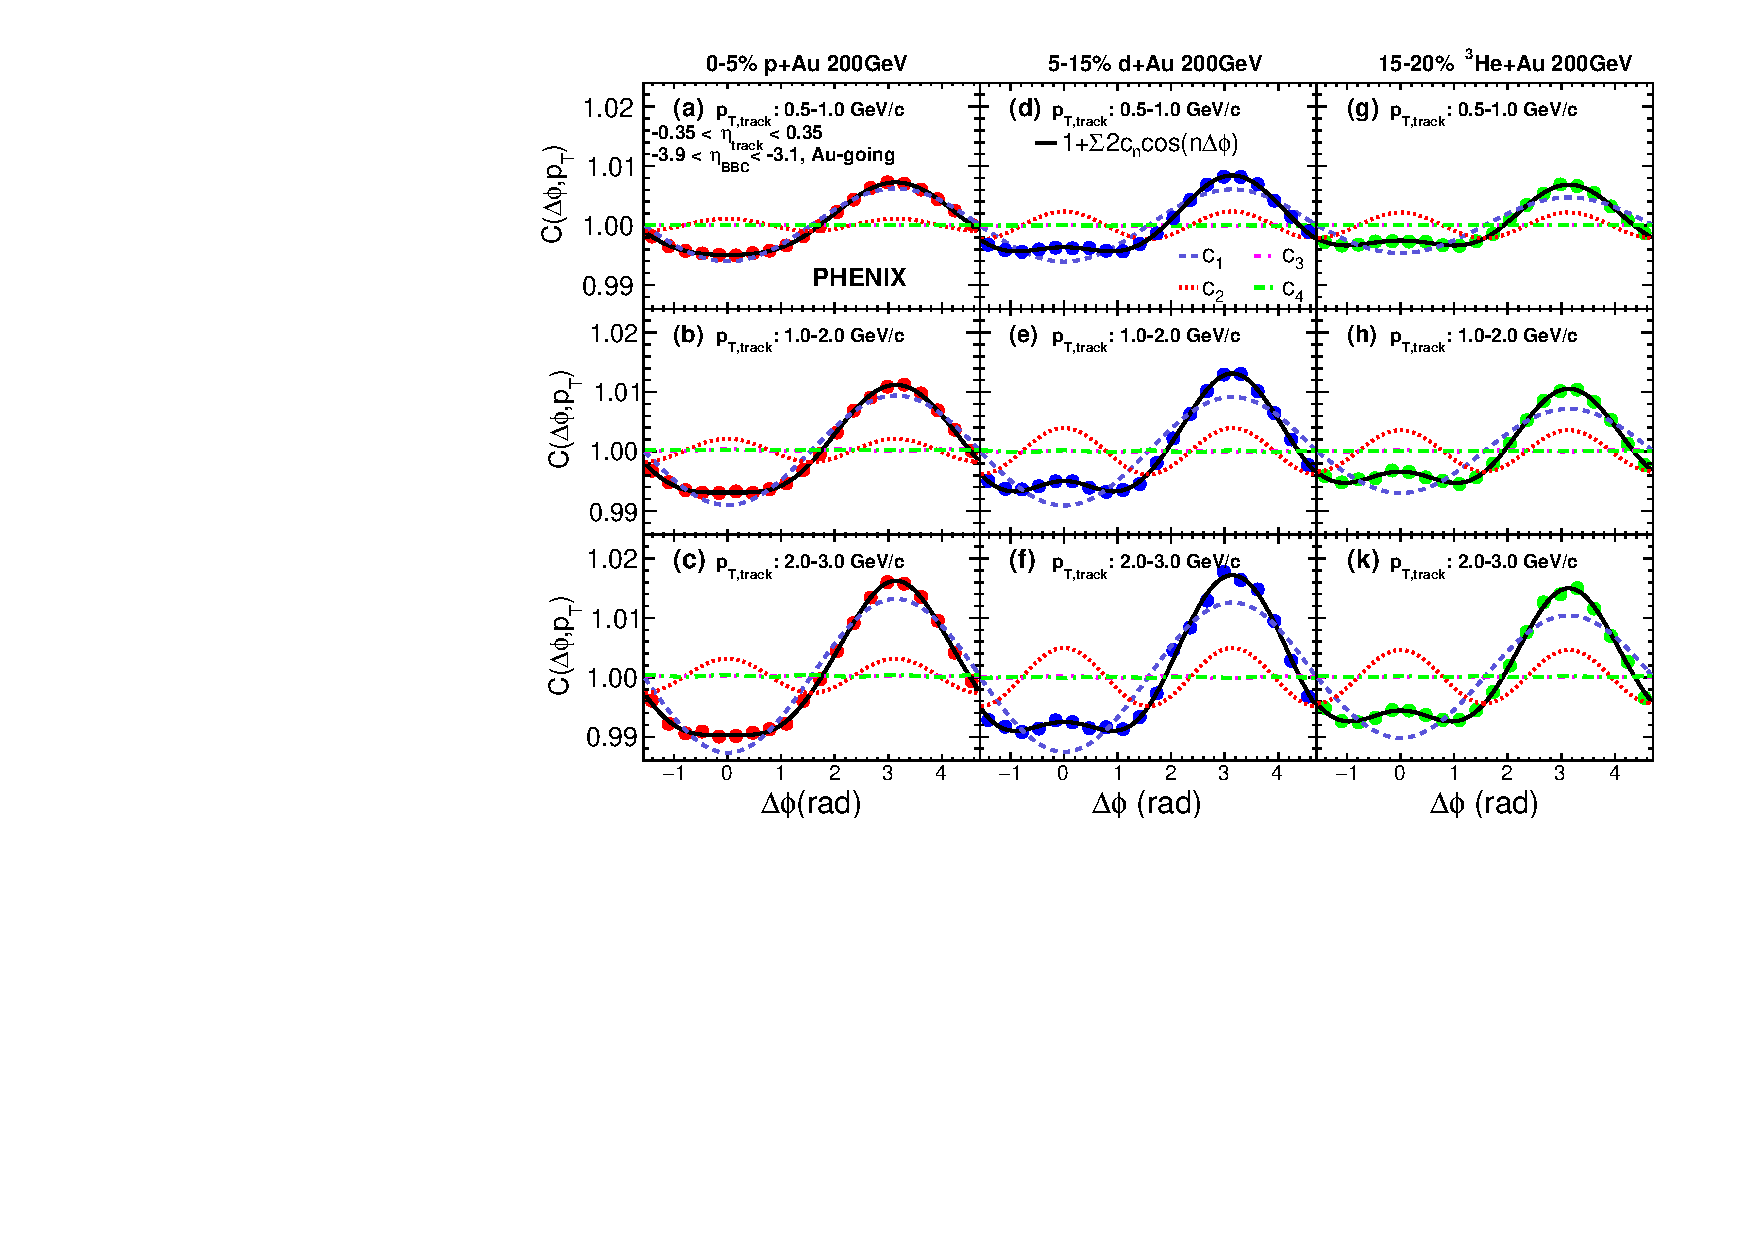
\includegraphics[scale=0.8]{Figures/figure1.pdf}
  \caption{(Color online) Azimuthal correlations $C(\Delta\phi,p_{T})$, as defined in
Eq.~\ref{eq:def_corr_function}, for track-BBC PMT pairs with different
track \pt selections in 0\%--5\% \pau collisions (left), 5\%--15\% \dau collisions (center) and
10\%--15\% \hau collisions (right) at \sqsn~=~200~GeV. From top to bottom,
the track \pt bins are 0.5--1.0, 1.0--2.0, and 2.0--3.0~GeV/$c$. Each
correlation function is fit with a four-term Fourier cosine series. The
individual harmonics from $n=1$ to $n=4$ are shown on each panel (dashed lines), along
with the fit function sum (solid line).}
\label{fig:figure1}
\end{figure*}

To study the effect of initial geometry and rule out any multiplicity effects on these long range angular correlations, we compare the correlation in 0\%--5\% \pau to those from 5\%--15\% \dau and 10\%--15\% \hau collisions, all corresponding to a similar mean BBC multiplicity. The results are shown in Figure ~\ref{fig:figure1}. A near-side peak is clearly visible in the 5\%--15\% \dau and 10\%--15\% \hau collisions, but not in the 0\%--5\% \pau. This indicates that the near-side peak is related to the initial geometry, since the eccentricity for 5\%--15\% \dau and 10\%--15\% \hau collisions is larger than that of 0\%--5\% \pau. We fit the correlations with a four-term Fourier cosine expansion. The second components ($c_{2}$) of the fits are shown in Fig.~\ref{fig:figure2}.
%%need the eccentricity

\begin{figure}[htbp]
  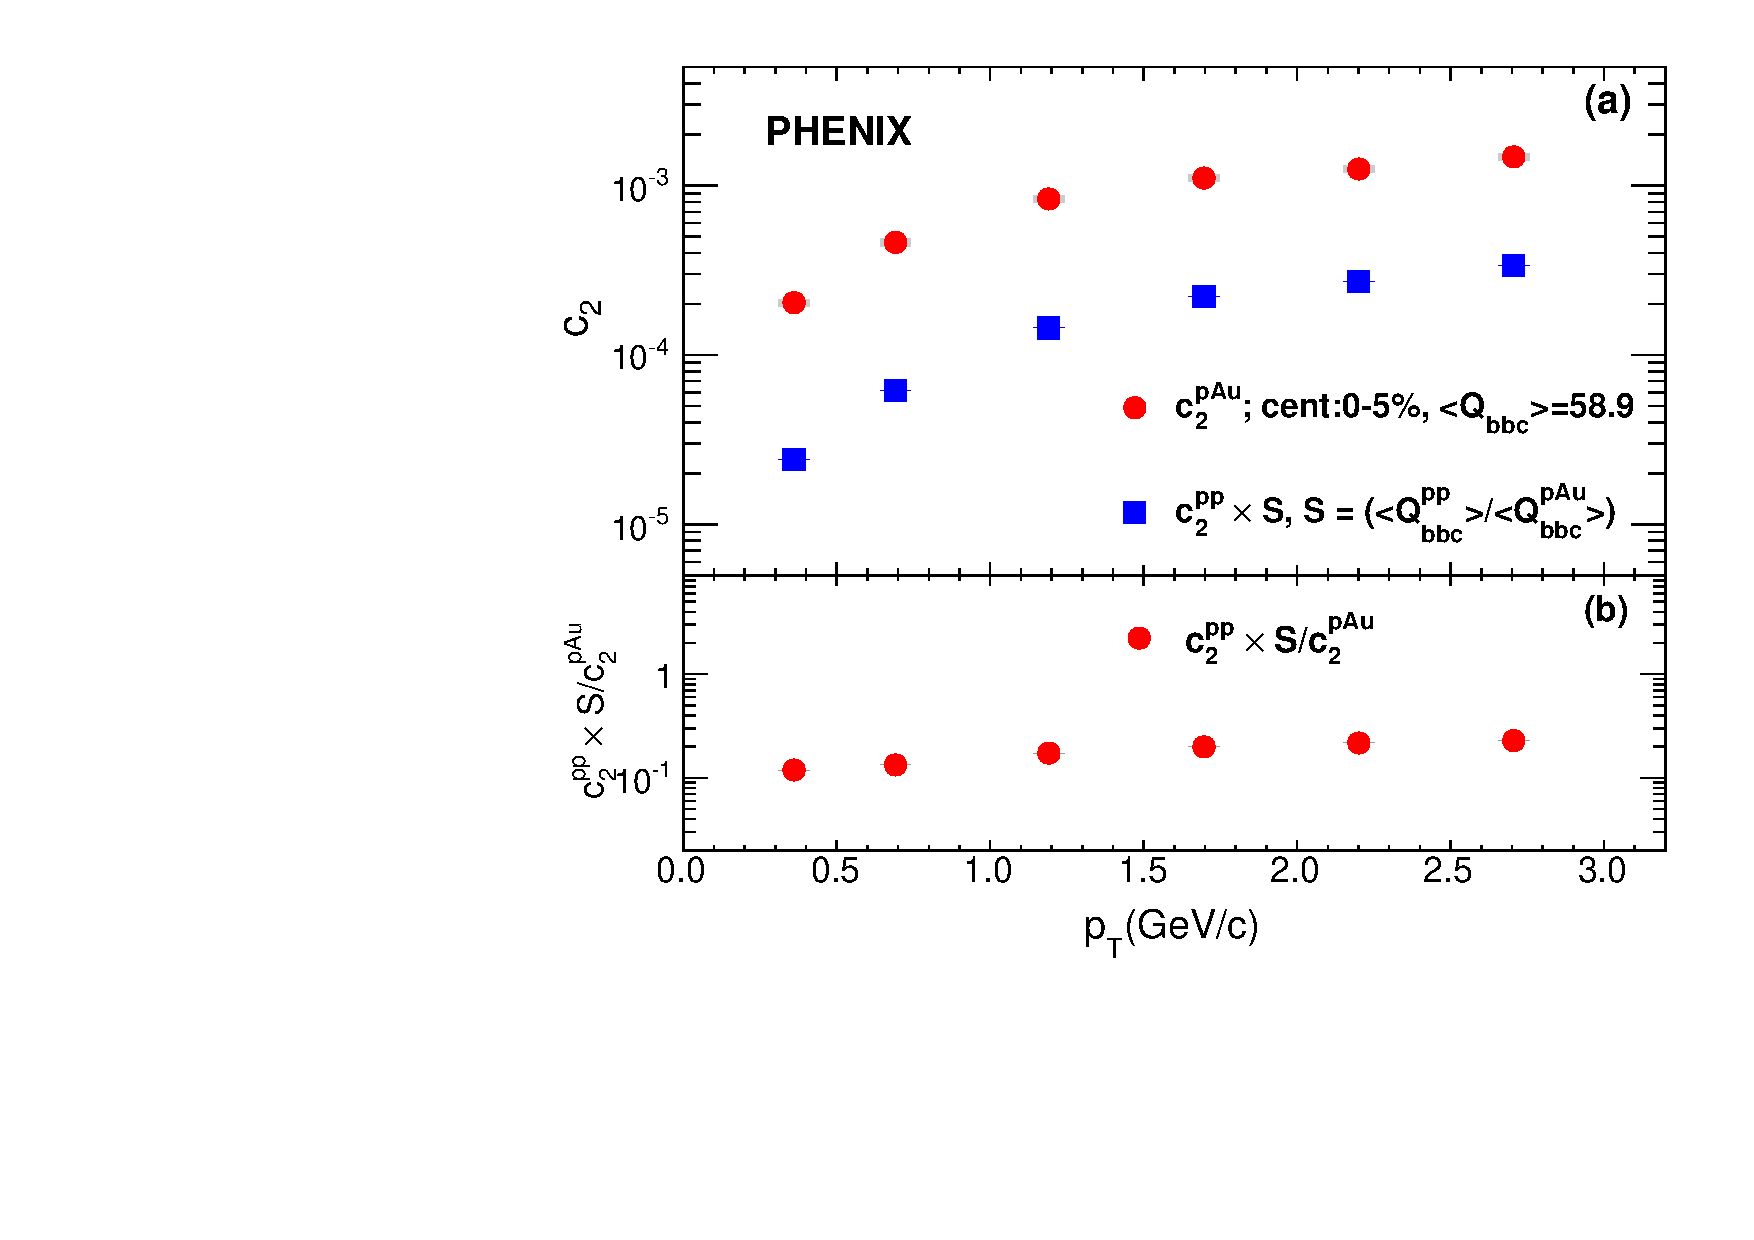
\includegraphics[scale=0.45]{Figures/figure2.pdf}
  \caption{(Color online)~The $c_2(p_T)$ coefficients for track-BBC pairs from 
0\%--5\% \pau, 5\%--15\% \dau and 10\%--15\% \hau collisions and
$c_{2}(p_{T})$ for pairs in minimum bias \pp collisions times the dilution
factor $\left( \sum Q^{{\rm BBC-S}} \right)_{p+p} / \left( \sum Q^{{\rm
BBC-S}} \right)_{{\rm pAu}}$ (open, denoted ``$c^{{\rm B}}$'' ). (b)~The
ratio $c^{{\rm B}}/c^{{\rm A}}$ is shown with statistical error bars.
}
\label{fig:figure2}
\end{figure}

Panel (a) of Fig.~\ref{fig:figure2} shows the $c_{2}$ coefficients from correlations measured in \pau, \dau and \hau. The $c_2$ values from 5\%--15\% \dau and 10\%--15\% \hau collisions are found to be comparable, and over fifty percent greater than those from 0\%--5\% \pau, with this difference being more pronounced at low \pt.

The correlation strength arising from elementary processes (e.g., jet fragmentation, resonance decays) across collision systems can be estimated quantitatively using published $c_{2}$ measurements in \pp collisions~\cite{PhysRevLett.115.142301}. These must be scaled down to account for the greater number of collisions within a single $(p,d,^{3}\text{He})+$Au event compared to \pp. This scale factor is taken to be the ratio of the total charge measured in the BBC-S $Q^{{\rm BBC-S}}$, as shown in Eq.~\ref{eq:dilute},

\begin{equation}
c_{n}^{{\rm pAu \; elementary}}(p_{T}) \simeq c_{n}^{p+p}(p_{T})
\frac{\left( \sum Q^{{\rm BBC-S}} \right)_{p+p}}
{\left( \sum Q^{{\rm BBC-S}} \right)_{{\rm pAu}}
}.
\label{eq:dilute}
\end{equation}
As is shown in panel (b) of Fig.~\ref{fig:figure2}, the relative
correlation strength in \pau from elementary processes is less than 25\%
at the highest \pt. In the case of \dau and \hau, such contributions
do not exceed 15\%. As a result, the $c_2$ from \dau and \hau collisions will be greater than that of \pau
even after subtracting the contributions from elementary processes.

Having accounted for elementary process contributions, $v_2$ is computed following the methodology described in Ref.~\cite{Adare:2015ctn}. The event plane method~\cite{ep} is used to measure $v_{2}(p_{T}) = \langle\sum \cos 2(\phi_{Particle}(p_{T})-\Psi^{Obs}_{2})\rangle/Res(\Psi^{Obs}_{2})$ for charged hadrons at midrapidity in central \pau events. The average is taken over particles in the same \pt bin and centrality.
As previously stated, the second order event plane $\Psi^{Obs}_{2}$ is measured for every event using the BBC-S and FVTX subsystems. Their difference is around a few percent, increasing to 12\% at $p_T\approx$ 3 GeV/c. This analysis uses the event plane measured with the FVTX, treating the difference with the BBC event plane as part of the systematic uncertainties. Sources of systematic uncertainties include: (1) track backgrounds from weak decays and photon conversions; (2) multiple collisions in a bunch crossing (i.e., event pile-up); (3) elementary process contributions. Their magnitude is quantified as follows: (1) the track background contribution is estimated by reducing the spatial matching windows in the PC3 from $3\sigma$ to $2\sigma$, finding a fractional change of 1\% in the measured $v_{2}$; (2) the pile up fraction is found to be less than 3\%, and a $^{+0}_{-3}\%$ asymmetric systematic uncertainty is assigned, since the $v_{2}$ from pile-up events is expected to be smaller; (3) The contribution from elementary processes can be estimated from Figure \ref{fig:figure2}, which reaches a maximum of 25\% at the highest $p_T$. We assign a $^{+0}_{-25}\%$ asymmetric systematic uncertainty since these elementary processes result in an enhanced $v_2$ signal as shown in Figure~\ref{fig:figure3}.

% \color{red}
% The $\Psi^{Obs}_{2}$ are corrected for each detector with a standard event-plane flattening technique \cite{REF MISSING} to remove the effect of any small, residual non-uniformity in the detector response. As a crosscheck we use event planes from both the full FVTX-S covering $−3.0 < \eta < −1.0$ and a subsection covering $−2.5 < \eta < −1.5$. The choice of the latter is to avoid edge effects and still retain good FVTX-S acceptance.We calculate the resolutions $\Psi^{Obs}_{2}$ for each detector using the standard three-event-plane method\cite{REF MISSING}, combining two event planes with the second order event plane determined from central-arm tracks, restricted to low \pt ($0.2 < \pt < 2.0$ GeV/c) to minimize contribution from jet fragments. %The values for the resolution obtained in both methods are round to be consistent within uncertainties. The event plane resolutions for each detector and order are shown in Table II.
% The $v_{2}$ measured in \pau using the three event planes described above are shown in fig. \ref{fig:figure3}. The main sources of systematic uncertainty for the $v_{2}$ measurements are: (1) track backgrounds from weak decays and photon conversions; (2) multiple \pau collisions in a bunch crossing (pile-up); (3) biases in event plane determination; and (4) elementary process/nonflow correlations. We assign the following values to account for these systematic uncertainties: (1) We estimate the track background contribution by reducing the spatial matching windows in PC3 from $3\sigma$ to $2\sigma$, and find a change of 1\% fractionally in $v_{2}$. (2) We expect the $v_{2}$ from pile-up events to be modestly reduced. Conservatively assuming that pile-up events that contaminate the sample at the level of 3\% have a negligible $v_{2}$, this results in a $^{+0}_{-3}\%$ systematic uncertainty. (3) Event plane effects are estimated from $v_{2}$ measurements using different event plane detectors show about 12\% for $v_{2}$. (4) The contribution from nonflow correlations at each \pt is estimated from Fig. \ref{fig:figure3}, reaching a maximum of 25\% $v_{2}$ in central \pau. We do not attempt to correct for this contribution and instead treat it as a systematic uncertainty. All of these contributions are summed in quadrature.
\color{black}

The possibility of comparing three collision systems with intrinsically different geometries provides a valuable opportunity to quantitatively study the effect of initial geometry. If we compared $v_2$ from different systems in the \emph{same} centrality, total particle production would scale with the size of the system, impacting the measured signal. 
Hence, selecting multiplicity-matched centrality classes allows for a controlled comparison of $v_2$ across systems. Figure~\ref{fig:figure3} shows the $v_2(\pt)$ measured in 0-5\% \pau, 5-15\% \dau, and 15-20\% \hau collisions using the same methodology. In all cases, there is a substantial $v_2$ that rises with \pt. The ordering of the curves directly correlates with the ordering of initial eccentricities $\varepsilon_2$, as presented in Table~\ref{table_geometry}. Namely, \dau has the highest $\varepsilon_2$, but close to that of \hau, while \pau has a much lower eccentrgicity than the other two systems. These results are consistent with a physical picture of small systems where initial geometry is the driver of final-state momentum anisotropy. However, if the $v_2$ results are divided by their corresponding $\varepsilon_2$ from Table~\ref{table_geometry}, they do not collapse to a common value as would be expected from a perfect geometric scaling. This behavior is shown in Figure~\ref{fig:figure3_epsilonratio}.

\begin{figure}[htbp]
  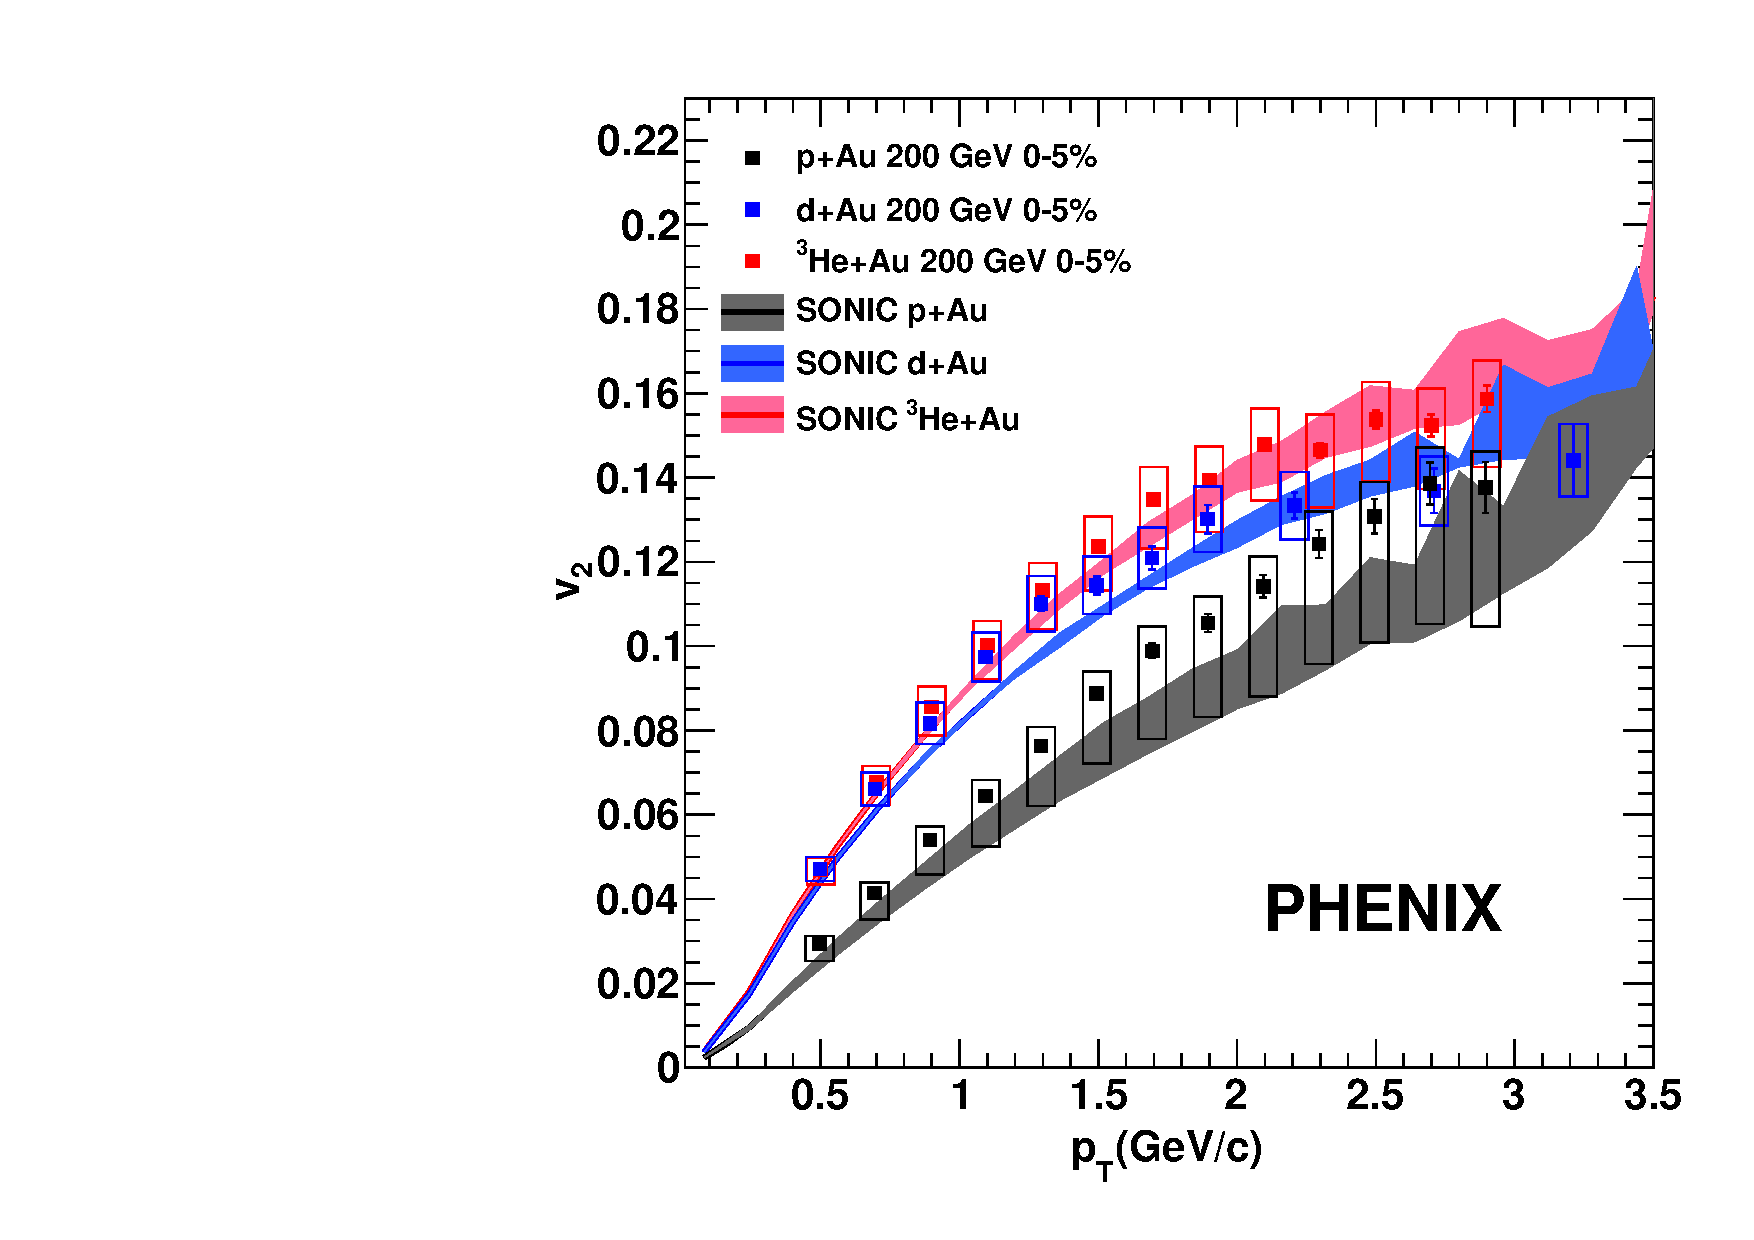
\includegraphics[scale=0.45]{Figures/figure3.pdf}
  \caption{(Color online)$v_2$ of charged hadrons within $|\eta| <$ 0.35 in 0\%--5\% \pau, 5\%--15\% \dau and 10\%--15\% \hau collisions, corresponding to similar multiplicity classes.}
\label{fig:figure3}
\end{figure}

\begin{figure}[htbp]
  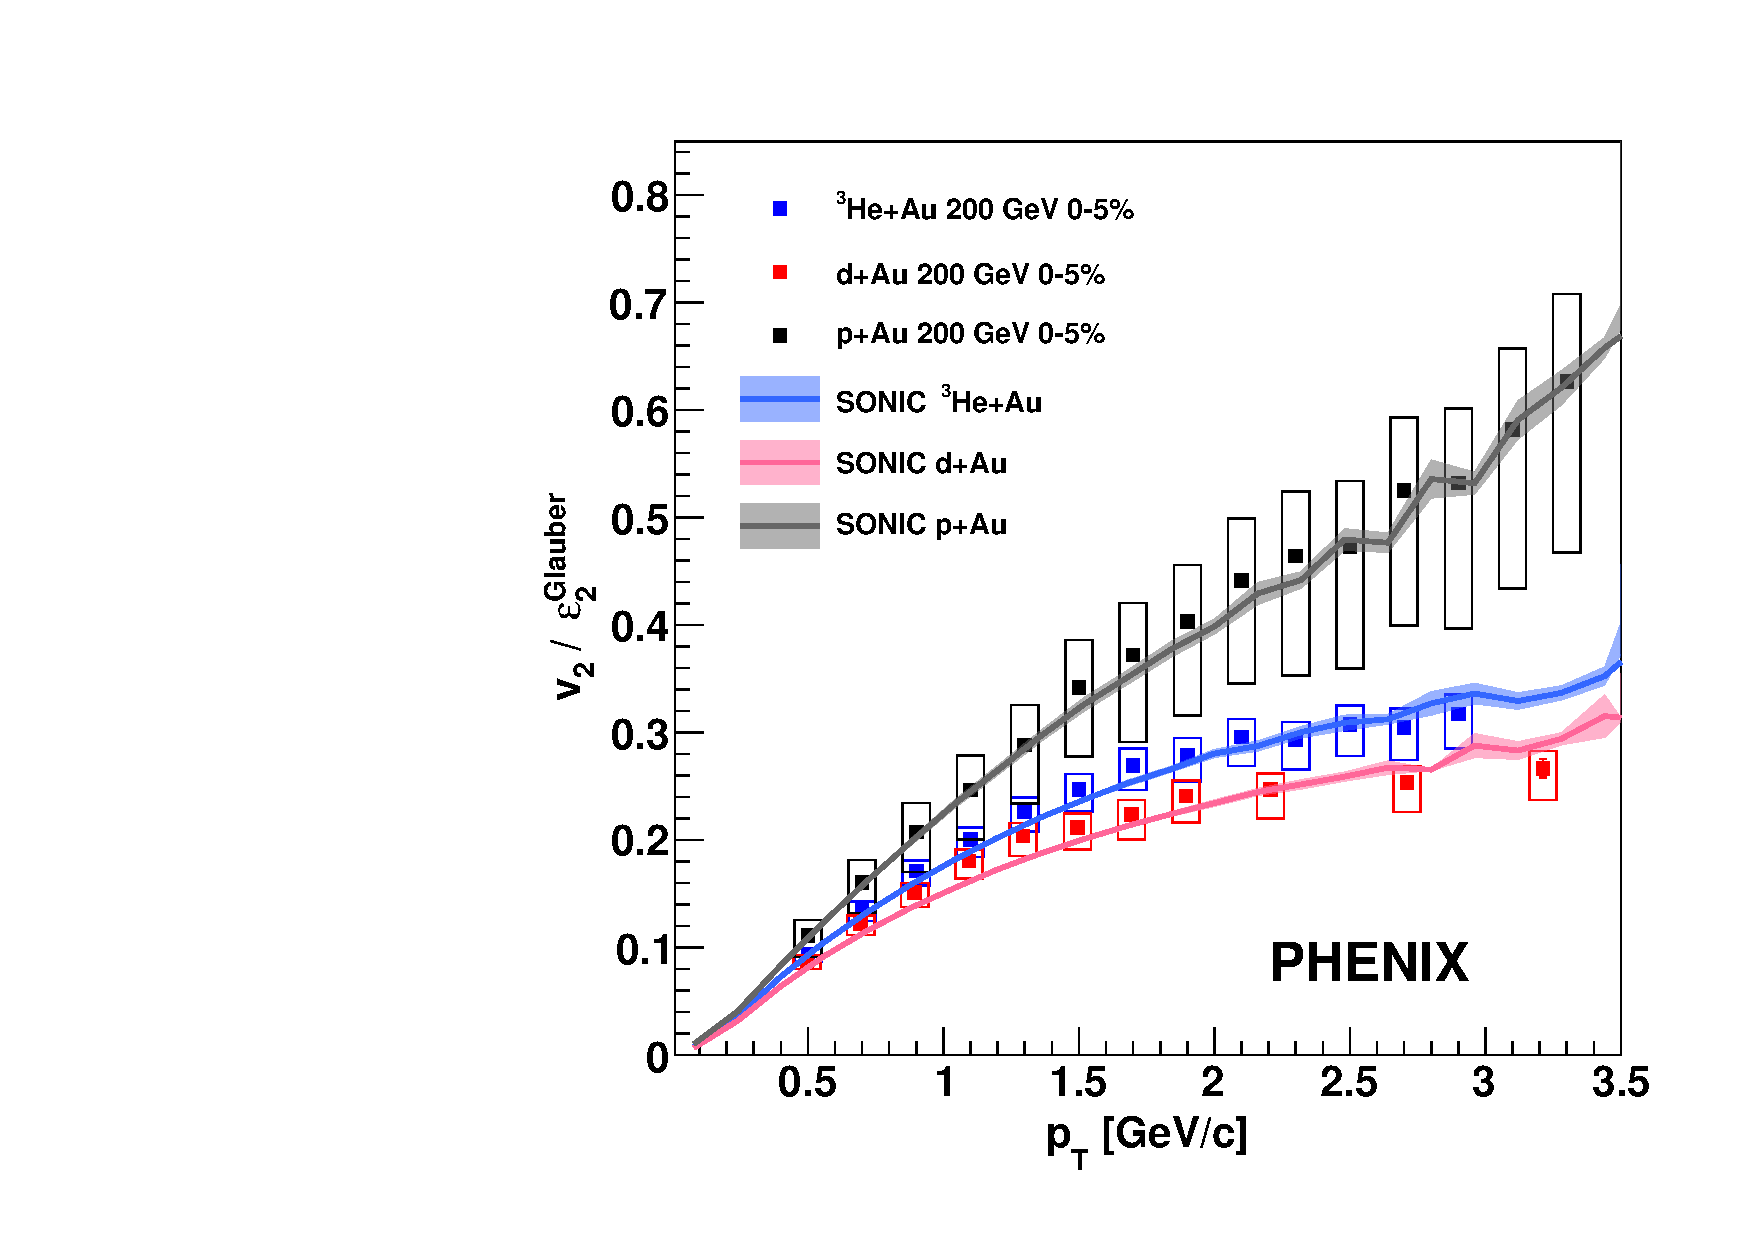
\includegraphics[scale=0.45]{Figures/figure3_epsilon2ratio.pdf}
  \caption{(Color online)$v_2$ of charged hadrons within $|\eta| <$ 0.35 in 0\%--5\% \pau, 5\%--15\% \dau and 10\%--15\% \hau collisions, divided by their corresponding eccentricity $\varepsilon_2$ from Glauber calculations.}
\label{fig:figure3_epsilonratio}
\end{figure}

%%%%%%  Main figure with final results and theory curves
%%%give this part to Javier for theory comparisons
In addition to confirming the importance of initial geometry, the results in Figure~\ref{fig:figure3} and their imperfect geometric scaling provide a stringent test for any theoretical model attempting to describe small system collectivity. Figure~\ref{fig:figure4} shows $v_2(\pt)$ for 0-5\% central \pau, \dau, and \hau events, for which theoretical predictions are available in the literature, most notably from hydrodynamics with Glauber initial conditions (\textsc{sonic}~\cite{Habich:2014jna} and \textsc{supersonic}~\cite{Romatschke:2015gxa}), hydrodynamics with IP-Glasma initial conditions~\cite{Schenke:2014gaa}, and A-Multi-Phase-Transport Model (\textsc{ampt})~\cite{lin_multiphase_2005}.

\begin{figure*}[htbp]
  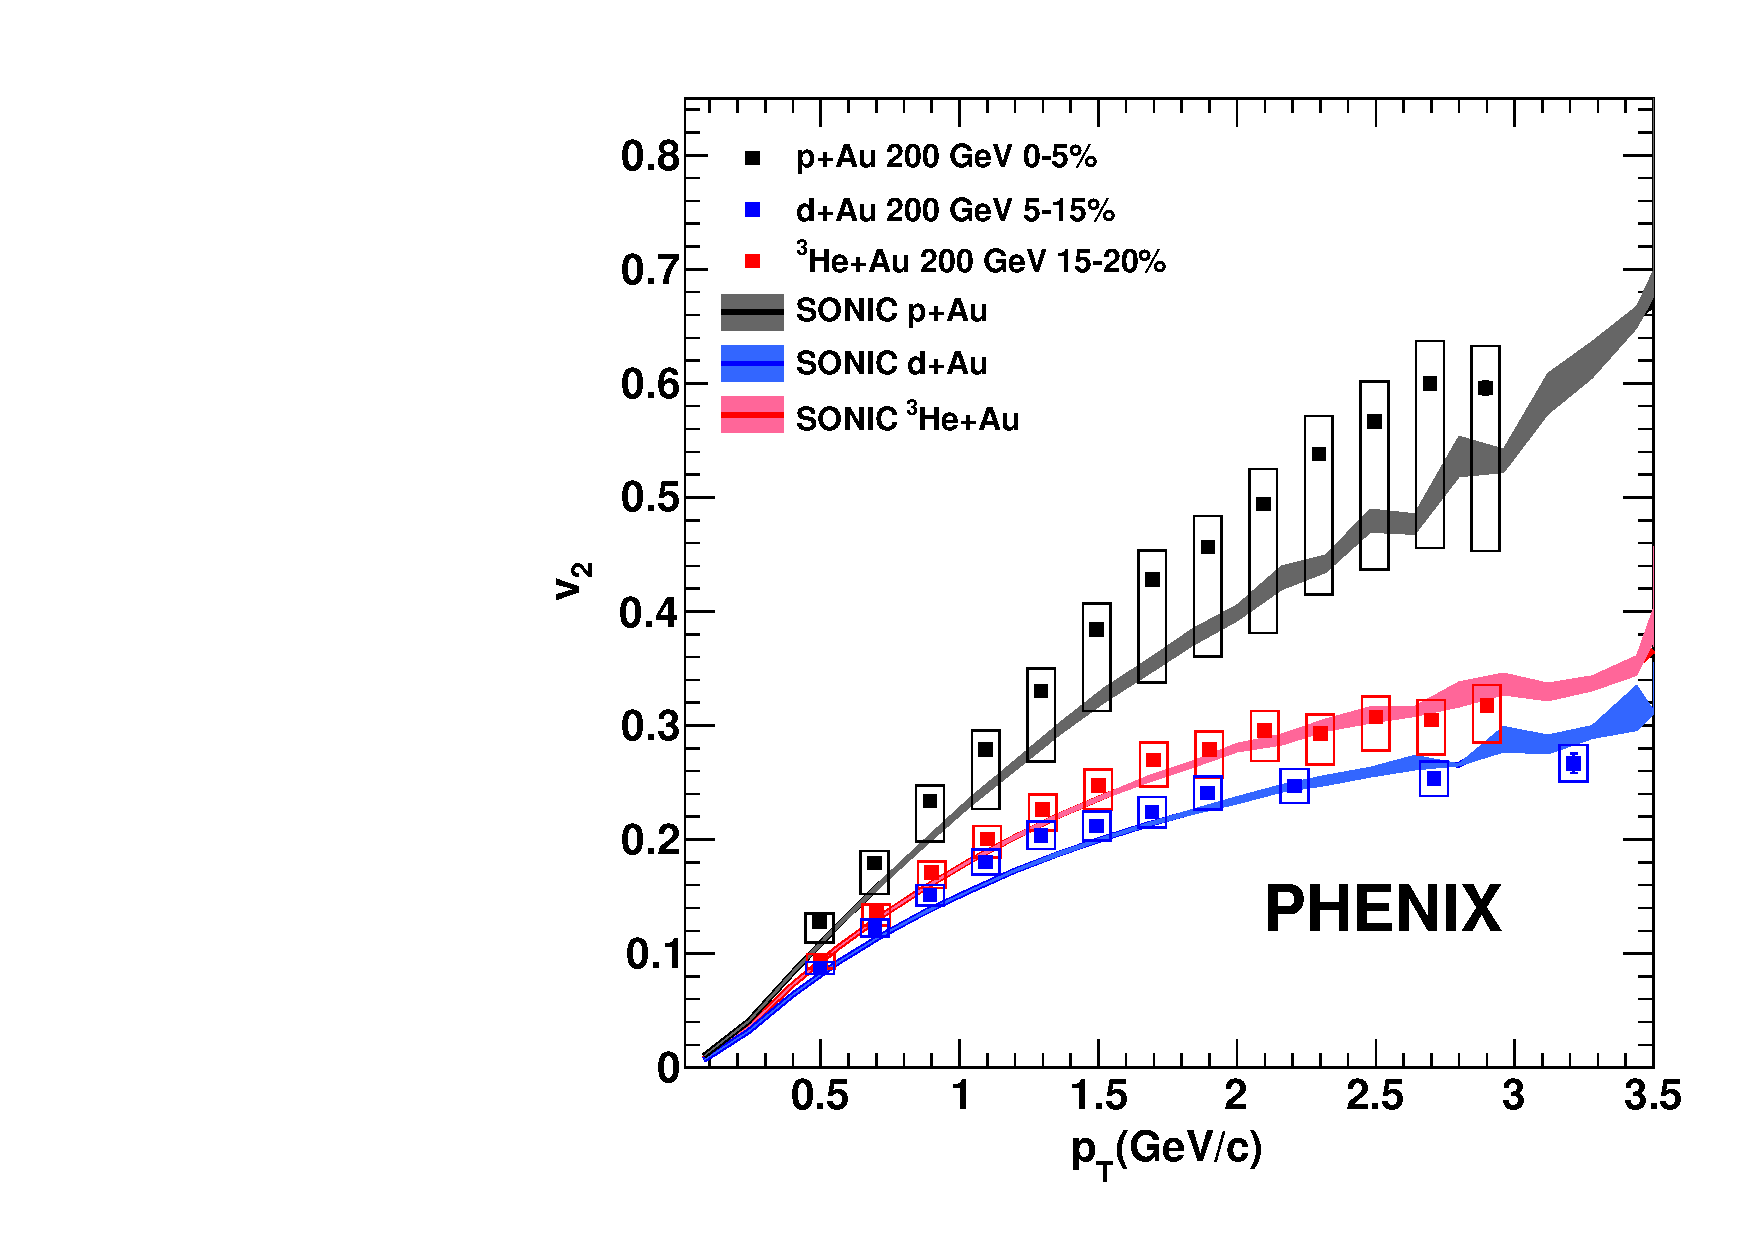
\includegraphics[scale=0.9]{Figures/figure4}
  \caption{(Color online) Transverse momentum dependence of $v_2$ in central 0-5\% (a) \pau, (b) \dau, and (c) \hau collisions at \sqsn = 200 GeV. Theoretical calculations from \textsc{ampt}, \textsc{(super)sonic}, and IPGlasma+Hydro are shown in each panel.}
%%Results for $v_{2}$ (circles) and $v_{3}$ (squares) as a function of \pt
%%for inclusive charged hadrons at mid-rapidity in 0\%--5\% central \heau
%%collisions at \sqsn~=~200~GeV; error bars are statistical and shaded bars
%%are systematic uncertainties as described in the text. Also shown are
%%various theoretical calculations, see text for details and references.}
\label{fig:figure4}
\end{figure*}

\begin{table}
\caption{Geometric characterization of small systems at \sqsn = 200 GeV for 0-5\% centrality from IP-Glasma initial conditions, and Monte Carlo Glauber initial conditions smeared with a two-dimensional Gaussian of width $\sigma=0.4$ fm.}
\begin{ruledtabular}
\begin{tabular}{c c c c}
\label{table_geometry_glasma}
 & \pau & \dau & \hau \\ \hline
 Glauber $\langle \varepsilon_2 \rangle$ & $0.231\pm 0.010$ & $0.540\pm 0.040$ & $0.504\pm 0.020$ \\
 IP-Glasma $\langle \varepsilon_2 \rangle$ & $0.099\pm 0.022$ & $0.595\pm 0.009$ & $0.555\pm 0.008$ \\
\end{tabular}
\end{ruledtabular}
\end{table}

The \textsc{sonic} and \textsc{supersonic} models incorporate standard Monte Carlo Glauber initial conditions followed by viscous hydrodynamics, and a transition to a hadronic cascade at T = 170 MeV. Furthermore, \textsc{supersonic} incorporates pre-equilibrium dynamics with a calculation in the framework of the AdS/CFT correspondence~\cite{vanderSchee:2013pia,Chesler:2015wra,Romatschke:2013re}. These two models agree well with the data within uncertainties, supporting the idea of initial geometry as the driver of the $v_n$ signal. Furthermore, this illustrates how these results impose useful constraints to reduce the number of \emph{free parameters} of the model, since many such parameters must be identical across systems, e.g., $\eta/s$, the transition temperature to a hadron cascade, and the nucleon cross section of $\sigma=0.4$ fm.

Predictions using IP-Glasma initial conditions followed by viscous hydrodynamics substantially overestimate the data for \dau and \hau, while underestimating it for \pau. This follows from the fact that IP-Glasma generates very \emph{circular} initial conditions for \pau, corresponding to very low $\varepsilon_2$ values; however, the presence of several hot spots in \dau and \hau result in IP-Glasma values for $\varepsilon_2$ more comparable to those from Glauber. This is shown in Table~\ref{table_geometry_glasma}. In the case of \dau and \hau, a better agreement with data can be achieved by increasing the value of $\eta$/s or by including a hadronic cascade stage. However, doing so would lower the prediction for \pau even further. This demonstrates that IP-Glasma does not generate the appropriate initial conditions to account for measured $v_n$ via hydrodynamic flow. 

It is important to notice that additional degrees of freedom on the geometry of \pau collisions arise from $x-$dependent fluctuations of the shape of the proton, as described in Ref.~\cite{Schlichting:2014ipa}. The contribution of this effect to the measured elliptic flow must be constrained by $p+p$ data, and also possibly by varying the target in other $p+$A systems.

Finally, \textsc{ampt} combines partonic and hadronic scattering in a single model. Using the initial Glauber geometry information to compute $v_2$ relative to the participant plane~\cite{Koop:2015wea} yields results that agree reasonably well with the data below $\pt \approx 1$ GeV/c, yet underpredict them at higher \pt. It is noteworthy that despite the very different physics of \textsc{ampt} compared to the other models, it has successfully been applied to a variety of systems at RHIC~\cite{Adare:2015cpn,Koop:2015wea}, and small systems at the LHC~\cite{ma_long-range_2014,ma_long-range_2014}.

We have presented results on azimuthal anisotropies and elliptic flow in central \pau at \sqsn = 200 GeV, compared with $v_2$ in \dau and \hau at similar multiplicities. These results impose strong constraints on models attempting to describe the formation and behavior of hot nuclear matter in small systems. We observe a clear---albeit imperfect---scaling of $v_2$ with $\varepsilon_2$, providing strong evidence for initial geometry as the source of final-state momentum anisotropies in these systems. This necessarily precludes other explanations based on initial-state momentum space domain effects. Calculations from \textsc{sonic} and \textsc{supersonic} are able to reproduce the measured $v_2$ and their scaling behavior for central events in all systems, thus establishing hydrodynamics as a valid model to understand the physics of collectivity in this regime. 

\bibliography{references}
\end{document}
%
% ****** End of file apssamp.tex ******